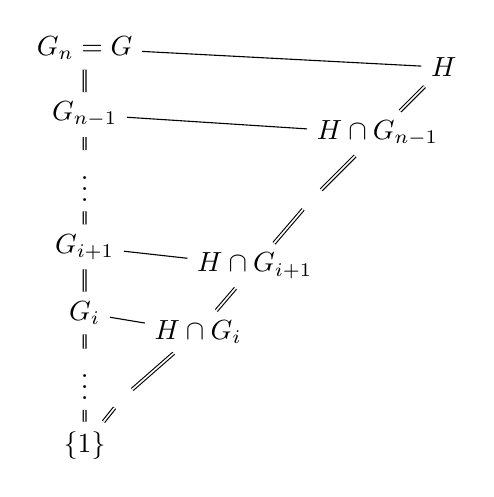
\begin{tikzpicture}[scale=1.2]
  % Nodes
  \node (Gn) at (-1,2.1) {$G_n=G$};
  \node (Gn-1) at (-1,1.4) {$G_{n-1}$};
  \node (p1) at (-1,0.7) {$\vdots$};
  \node (Gi+1) at (-1,0) {$G_{i+1}$};
  \node (Gi) at (-1,-0.7) {$G_i$};
  \node (p2) at (-1,-1.4) {$\vdots$};
  \node (1) at (-1,-2.1) {$\{1\}$};
  \node (H) at (2.8,1.9) {$H$};
  \node (HGn-1) at (2.1,1.2) {$H\cap G_{n-1}$};
  \node (p3) at (1.4,0.5) {$\iddots$};
  \node (HGi+1) at (0.8,-0.2) {$H\cap G_{i+1}$};
  \node (HGi) at (0.2,-0.9) {$H\cap G_i$};
  \node (p4) at (-0.6,-1.6) {$\iddots$};

  % Lineas nodos
  \draw[double] (Gn) -- (Gn-1);
  \draw[double] (Gn-1) -- (p1);
  \draw[double] (p1) -- (Gi+1);
  \draw[double] (Gi+1) -- (Gi);
  \draw[double] (Gi) -- (p2);
  \draw[double] (p2) -- (1);
  \draw (Gn) -- (H);
  \draw (Gn-1) -- (HGn-1);
  \draw (Gi+1) -- (HGi+1);
  \draw (Gi) -- (HGi);
  \draw[double] (H) -- (HGn-1);
  \draw[double] (HGn-1) -- (p3);
  \draw[double] (p3) -- (HGi+1);
  \draw[double] (HGi+1) -- (HGi);
  \draw[double] (HGi) -- (p4);
  \draw[double] (p4) -- (1);
\end{tikzpicture}
